\chapter{Implementing the GUI}

I've chosen the \emph{Simple and Fast Multimedia Library}
\href{https://www.sfml-dev.org/index.php}{SFML} for creating the graphical user interface
of the app.
It lives up to its name and is available on all major platforms and programming languages.

In this chapter we'll learn how to display the board and the chess pieces on it.
In order to show valid moves for each piece, we will also learn the basic rules of the game.

I'm using \href{https://cmake.org/}{CMake} for building the C\textsuperscript{++} code,
and the SFML CMake project template, which will build the SFML libraries.
So you will need to have the following components installed on your machine:

\begin{itemize}
  \item a decent C\textsuperscript{++} compiler (any of the major compilers will do)
  \item the \emph{git} tool
  \item the \emph{cmake} tool
  \item the required system packages for
    \href{https://www.sfml-dev.org/tutorials/2.6/start-cmake.php}{SFML}
\end{itemize}
 
On a linux system, all those components can be installed with your systems package manager
(e.g. with \texttt{apt-get} on Ubuntu).
The same is true for Mac OS, just use the included \texttt{clang++} compiler and install
missing components with \href{https://brew.sh/}{homebrew}:
\texttt{<brew install git cmake sfml>}.

When everything is in place, just clone my repository with\\
\texttt{<git clone https://github.com/okrischer/ThinkChess.git>} and execute\\
\texttt{<cmake -B build>} from the root folder of your local copy.\\
If everything went well, change to the \texttt{build} folder and execute
\texttt{<cmake --build .>} and voila, you have a simple chess app, which you can start with
\texttt{<./ThinkChess>}.

I strongly encourage you to code all the following steps with an editor of your choice
for yourself and see if you can get the code running. Nothing is gained if you just skim
over the provided source code.

If you have \LaTeX\ installed on your machine, you can also build the documentation
with \texttt{<pdflatex -shell-escape Main.tex>} from the \texttt{doc} folder,
which will produce this document.

\section{Displaying the board and the pieces}

Let's start with the basic framework for displaying something with SFML:

\begin{cpp*}{linenos}
#include <SFML/Graphics.hpp>

int main() {
  sf::ContextSettings settings;
  settings.antialiasingLevel = 8;
  auto window = sf::RenderWindow{ {640u, 640u}, "Think Chess",
              sf::Style::Default, settings };
  window.setFramerateLimit(10);

  while (window.isOpen()) {
    for (auto event = sf::Event{}; window.pollEvent(event);) {
      if (event.type == sf::Event::Closed) {
        window.close();
      }
    }
    window.draw(bs);
    window.display();
  }
}
\end{cpp*}

This is the main file for our app (\texttt{app/main.cpp}).
Thus, it defines the \mintinline{cpp}{int main()} function (3) as the starting point of the app.
The numbers in paranthesis \texttt{(x)} always refer to the last code snippet.\\
In order to access SFML functionality, we have to \mintinline{cpp}{#include} the SFML Graphics
library (1), which was built by \emph{cmake}.\\
First, we define the context (4) and set the antialiasing level to 8 within the context (5).\\
Next, we define the main window for our app (6), setting its size, title, style, and the context
settings.\\
Then we set the framerate to 10 (8), i.e. 10 frames per second; we don't need more
for such a static app, and the app will keep responsive with that.\\
Next comes the central part: entering the main game loop (10-18). The game loop usually contains
three steps:

\begin{enumerate}
  \item an event loop, processing all user inputs for the current frame (11-15)
  \item several drawing instructions (16) for all items to appear in the frame
  \item a call to \mintinline{cpp}{window.display()}, which causes all drawn elements to be
    actually displayed.
\end{enumerate}

But we don't have anything to draw yet; let's change this by adding a chessboard
within the main function, just before entering the game loop (9):

\begin{cpp*}{linenos}
  sf::Texture bi;
  bi.loadFromFile("../img/chessboard.jpg");
  sf::Sprite bs;
  bs.setTexture(bi);
\end{cpp*}

Here, we create a SFML texture (1) and load an image from the file system into that texture (2).
Then we create a SFML sprite (3) and set its texture  to that image (4).

If you run the app now, you would see an empty chess board:

\begin{center}
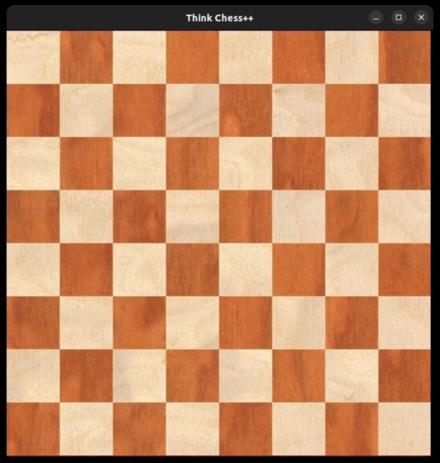
\includegraphics[width=.5\linewidth]{../img/emptyBoard.jpg}
\end{center}

Not that interesting, so we're going to add the chess pieces at their initial position.
For that, let's introduce the pieces at first: they come in two colors, \emph{white}
and \emph{black}, each for one player, and they are called as follows
(from left to right in the image below):

\begin{center}

\includegraphics[width=.5\linewidth]{../img/figures.png}
\end{center}

\begin{enumerate}
  \item \emph{King} [-]
  \item \emph{Queen} [8]
  \item \emph{Bishop} [3]
  \item \emph{Knight} [3]
  \item \emph{Rook} [4]
  \item \emph{Pawn} [1]
\end{enumerate}

Every piece, except the king, has a value assigned to it; this is just by convention and
not necessary for the original game play.
The value shows the strength of the piece and serves for a basic evaluation of each players
position during the game.
So, the \emph{Queen} is the most powerful piece in the game, followed by the \emph{Rook}, and
the \emph{Bishop} and the \emph{Knight}, both of equal value.
The least worthy piece is the \emph{Pawn}.

But why has the \emph{King} no value assigned?\\
The goal of the game is to put your opponents \emph{King} in a position, where it is exposed
to a thread of beeing captured; this position is called \emph{check}.
If the threatened \emph{King} cannot respond to the \emph{check} in the very next move,
the game is over, and your opponent has lost the game.
This position is called \emph{checkmate}.
So, the \emph{King} is never actually captured, it stays on the board until the end of the game.
Because of this, it doesn't make any sense to give him a value for evaluating a players position. 

We'll cover the movement of the pieces in great detail in the next section~\ref{sec:validmoves}.
But, for now, let's concentrate on how to display the pieces:

\begin{cpp*}{linenos}
  sf::Texture figures;
  figures.loadFromFile("../img/figures.png");

  sf::Sprite wk;
  wk.setTexture(figures);
  wk.setTextureRect(sf::IntRect(0,0,60,60));

  sf::Sprite bk;
  bk.setTexture(figures);
  bk.setTextureRect(sf::IntRect(0,60,60,60));
  // --- snip ---
\end{cpp*}

We have loaded a texture, containing the figures of all pieces (2).
Then we define distinct sprites for every piece, calling them \emph{wk} for the white king (4),
\emph{bk} for the black king (8), and so forth.\\
Finally, we cut out the matching parts of the \mintinline{cpp}{figures} texture and assign
them to every distinct sprite (6, 10).


Notice, that I've taken care that all the sprites have the same size of
$60 \times 60$ pixels.
As the board has a size of $640 \times 640$ pixels, containing $8 \times 8$ light and dark squares,
every square on the board has a size of $80 \times 80$ pixels.
That allows us to place the sprites evenly on the board with an offeset of 10 pixels to the
boundary of each square.

In order to actually place the pieces on the board, we need a data structure, being able to
keep track of the 64 squares.
As it turns out, an $8 \times 8$ vector matrix is a good fit for that:

\begin{cpp}
std::vector<std::vector<Piece*>> board(8, std::vector<Piece*>(8));
\end{cpp}

You could have used any type of vector matrix for keeping track of the pieces,
but I've chosen an \emph{object-oriented} approach:
every piece is represented by a raw pointer (indicated with the *) to an instance of the
\mintinline{cpp}{class Piece}.
That allows for greater flexibility in implementing the game logic: instead of putting
the game logic in the main file, we are going to implement it in a new file \texttt{app/pieces.cpp}.

So, let's have a look on how \mintinline{cpp}{Piece} is actually implemented:

\begin{cpp}
#pragma once
#include <vector>

class Piece {
public:
  virtual ~Piece() {}
  virtual char getType() = 0;
  virtual char getValue() = 0;
  virtual bool isWhite() = 0;
  virtual bool isCaptured() = 0;
  virtual std::vector<std::vector<short>>
    validMoves(std::vector<std::vector<Piece*>>& bd) = 0;
};
\end{cpp}

As you may have guessed, this code snippet is not from the \texttt{pieces.cpp} file, but from its
\emph{header} file, located at \texttt{include/pieces.hpp}.
I've decided to separate the compilation units into a public interface (the header file) and
an implementation file.
That allows to use the definitions of the header file in any other implementation file and
gives us even more flexibility in structuring the source code.

\mintinline{cpp}{Piece} is declared as a pure \emph{abstract} interface.
That means, it doesn't have a \emph{constructor}, and all the member functions are marked
as \mintinline{cpp}{virtual}.
Thus, you cannot instanciate it directly, and to make any use of it, we have to create
\emph{derived} classes (subclasses of \mintinline{cpp}{Piece}) for every piece, which will
implement the virtual functions.
The reason for doing so is: we need different implementations for performing moves for
each piece, but also a common type for storing them in the board matrix. 

The concrete types for \mintinline{cpp}{Piece} are implemented like so:

\begin{cpp*}{linenos}
class King : public Piece {
public:
  ~King() {}
  King(bool w, int r, int c) : type{'k'}, white{w}, value{0},
                              captured{false}, row{r}, col{c} {}

  char getType() override { return type; }
  char getValue() override { return value; }
  bool isWhite() override { return white; }
  bool isCaptured() override { return captured; }

  std::vector<std::vector<short>>
    validMoves(std::vector<std::vector<Piece*>>& bd) override;

private:
  char type;
  bool white;
  short value;
  bool captured;
  int row;
  int col;
};
\end{cpp*}

The other pieces are implemented likewise; the only difference between them so far is the
implementation of the member function \mintinline{cpp}{validMoves()} (12-13).
I decided to leave the class definitions in the header file, and to move only those different
implementations to the file \texttt{app/pieces.cpp}.
We'll study these implementations in the next section~\ref{sec:validmoves}.

For now, we are only interested in the class definitions:\\
each of them is derived from \mintinline{cpp}{class Piece} (1) and has a \emph{destructor} (3),
which will be called by the compiler when an instance of the class is destroyed.
This will happen automatically, whenever an \emph{automatic} variable gets out of scope.
But, if a reference to an instance was created explicitly (using the keyword \mintinline{cpp}{new}),
we have to \mintinline{cpp}{delete} that object explicitly in order to avoid \emph{memory leaks}.

Next, we have the \emph{constructor} (4-5):\\
it initializes the instance with its type (which we need only for drawing the correct sprite),
the color of the piece (white or black), its value, and the current position
of the piece (the row and column of the piece in the board matrix).

The following member functions (6-10) are just \emph{getters} to retrieve the
\mintinline{cpp}{private} member types.

With the derived \mintinline{cpp}{Piece} types in place, we can initially fill the board matrix:

\begin{cpp}
void reset_board(std::vector<std::vector<Piece*>>& bd) {
  for (auto rank : bd) {
    for (auto piece : rank) {
      delete piece;
    }
  }
  // rank 8 (black)
  bd[0][0] = new Rook(0,0,0);
  bd[0][1] = new Knight(0,0,1);
  bd[0][2] = new Bishop(0,0,2);
  bd[0][3] = new Queen(0,0,3);
  bd[0][4] = new King(0,0,4);
  bd[0][5] = new Bishop(0,0,5);
  bd[0][6] = new Knight(0,0,6);
  bd[0][7] = new Rook(0,0,7);
  // rank 7 (black)
  bd[1][0] = new Pawn(0,1,0);
  bd[1][1] = new Pawn(0,1,1);
  bd[1][2] = new Pawn(0,1,2);
  bd[1][3] = new Pawn(0,1,3);
  bd[1][4] = new Pawn(0,1,4);
  bd[1][5] = new Pawn(0,1,5);
  bd[1][6] = new Pawn(0,1,6);
  bd[1][7] = new Pawn(0,1,7);
  // rank 2 (white)
  bd[6][0] = new Pawn(1,6,0);
  bd[6][1] = new Pawn(1,6,1);
  bd[6][2] = new Pawn(1,6,2);
  bd[6][3] = new Pawn(1,6,3);
  bd[6][4] = new Pawn(1,6,4);
  bd[6][5] = new Pawn(1,6,5);
  bd[6][6] = new Pawn(1,6,6);
  bd[6][7] = new Pawn(1,6,7);
  // rank 1 (white)
  bd[7][0] = new Rook(1,7,0);
  bd[7][1] = new Knight(1,7,1);
  bd[7][2] = new Bishop(1,7,2);
  bd[7][3] = new Queen(1,7,3);
  bd[7][4] = new King(1,7,4);
  bd[7][5] = new Bishop(1,7,5);
  bd[7][6] = new Knight(1,7,6);
  bd[7][7] = new Rook(1,7,7);
}
\end{cpp}

That seems tedious, but thankfully we have to do this only once.
I've placed the initialization code within a function \mintinline{cpp}{void reset_board()},
just in case we want to reset the board later (e.g. when starting a new game).
The board is passed as an automatic reference to the function (indicated by the \& after the
parameter type), such that we are able to modify the board directly,
instead of working with a copy of the board.

The code in the first three lines actually resets the board by deleting all existing
references to pieces.
When setting the pieces, you have to be careful: every piece must be initialized with exactly the
same coordinates from the board (and of course with the correct color: 0 for black and 1 for white).

The rows of a chessboard are called \emph{ranks}, while the colums are called
\emph{files}.
The ranks are indicated by the numbers 1 to 8, whereas the files are indicated by the letters
\texttt{a} to \texttt{h}, both starting at the lower left square (the dark field \texttt{a1}):
\begin{verbatim}
8 . . . . . . . .
7 . . . . . . . .
6 . . . . . . . .
5 . . . . . . . .
4 . . . . . . . .
3 . . . . . . . .
2 . . . . . . . .
1 . . . . . . . .
  a b c d e f g h
\end{verbatim}

With the initialization code above, the pieces will be placed like so on the board:

\begin{verbatim}
8 R N B Q K B N R
7 P P P P P P P P
6 . . . . . . . .
5 . . . . . . . .
4 . . . . . . . .
3 . . . . . . . .
2 P P P P P P P P
1 R N B Q K B N R
  a b c d e f g h
\end{verbatim}

Observe that we abbreviate the \emph{Knight} with the letter \texttt{N} to avoid confusion with
the \emph{King}.
So, the white \emph{Queen} is placed at \texttt{d1}, the black \emph{Queen} at \texttt{d8},
and so forth.

Now we can use the filled board matrix to actually draw the pieces within the game loop of the
main function:

\begin{cpp*}{linenos}
    // draw board
    window.draw(bs);
    // draw pieces
    for (int row = 0; row < 8; row++) {
      for (int col = 0; col < 8; col++) {
        if (board[row][col]) {
          auto piece = board[row][col];
          sf::Sprite pc;
          switch (piece->getType()) {
          case 'k':
            piece->isWhite() ? pc = wk : pc = bk;
            break;
          case 'q':
            piece->isWhite() ? pc = wq : pc = bq;
            break;
          case 'r':
            piece->isWhite() ? pc = wr : pc = br;
            break;
          case 'b':
            piece->isWhite() ? pc = wb : pc = bb;
            break;
          case 'n':
            piece->isWhite() ? pc = wn : pc = bn;
            break;
          case 'p':
            piece->isWhite() ? pc = wp : pc = bp;
            break;
          }
          pc.setPosition(col*80.f + 10.f, row*80.f + 10.f);
          window.draw(pc);
        }
      }
    }
\end{cpp*}

We are iterating over all elements of the matrix and get the piece at this position (7).
Then we get the type and color of that piece by calling the appropriate getter functions
(\mintinline{cpp}{getType(), isWhite()}) on it, and let a newly created sprite \texttt{pc}
point to the corresponding figure sprite (9-28).
Finally, we set the correct postion of the \texttt{pc} sprite on the board (29) and draw it
to the current frame buffer (30).

And that's it: when you start the app now, you will see this screen, which shows a
correct initialized chessboard with all pieces:

\begin{center}
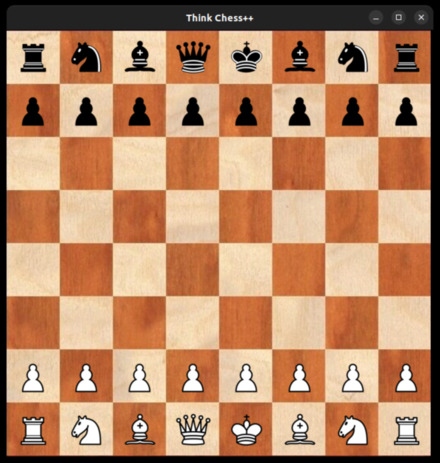
\includegraphics[width=.5\linewidth]{../img/boardWithPieces.jpg}
\end{center}


\section{Showing valid moves}\label{sec:validmoves}


